\documentclass[../main.tex]{subfiles}
\graphicspath{{\subfix{../img/}}}
\begin{document}
    
    In this section we are going to show with empirical evidence that, indeed, the mixing result found makes sense. In particular, we want to address the following questions: 
    
    \begin{itemize}
        \item To begin with, it is interesting to understand if mixing happens within the time limit set by Theorem \ref{theorem:mixing_theorem}. In particular, if the result is correct, the mixing time for the Lovasz-Simonovits curve should behave like $O\left(\frac{\log(\text{vol}(H))}{\phi^2}\right)$. Hence, by providing the algorithm a family of hypergraphs with constant volume and different conductance or vice versa, we should observe a mixing time logarithmic with respect to a change in the volume, and inversely quadratic when the conductance changes.
        
        \item In addition, we want to study empirically the following behaviour: in $r$-uniform hypergraphs, the theoretical upper bound according to \cite{continuous_laplacian_hypergraph} is dependent on $r$: in particular $t = O\left(\frac{\log(\text{vol}(H))}{\gamma_2}\right)$ $\leq O\left(\frac{\log(\text{vol}(H))}{r \phi^2}\right)$ (Thanks to the Hypergraph Cheeger’s Inequality theorem in \cite{Kapralov2020Nov}). Notice that, in contrast, the parameter $r$ disappears in our discussion (it is possible to see that by assuming that the hypergraph is $r$-uniform, the proof of Theorem \ref{theorem:mixing_theorem} cannot leverage such additional information). What we want to understand is whether the additional $r$ factor is important also in our analysis and it has been somehow overseen, or if the method is simply not powerful enough to explain a mixing time also dependent on $r$.
    \end{itemize}
    
    We start our discussion with the analysis of a family of hypergraphs with constant volume and varying conductance, and vice versa.
    
    In order to reproduce the experiments, you can use the code available on GitHub \footnote{https://github.com/steber97/spectral\_local\_clustering}
    
    \subsection{Generate a hypergraph with desired conductance}
    \label{subsec:generate_hypergraph_with_desired_conductance}
    
    
    	\begin{algorithm}
    		\label{algo:generate_hypergraph_with_desired_conductance}
    		\caption{Create hypergraph with desired conductance and volume}
    		\SetAlgoLined
    		\text{Requires: } $n \geq 0, \text{vol}(H), 0<\phi<1$ \\
    		\text{Returns: } $H: \phi(H) = \phi$ \\
    		$A := [1, ..., \frac{n}{2}]$ \\
    		$B := [\frac{n}{2}+1, ..., n]$ \\
    		$E := \emptyset$ \\
    		$\text{vol\_so\_far} := 0$ \\
    		\While{$|E| < \text{vol}(H) \frac{\phi}{2}$} 
    		{
    			$r$ = random(2, 1/$\phi$) \\
    			$e$ = $\{v: |e|=r, e\cap A \neq \emptyset \land e\cap B \neq \emptyset\}$ \\ 
    			$E = E \cup e$
    		}
    		$\text{vol\_bip} = \text{vol}(A)$\\
    		\While{vol($A$) $<$ vol($H$)/2}
    		{
    			$r$ = random(2, 1/$\phi$) \\
    			$e = \{v: |e|=r, e\cap A \neq \emptyset \land e\cap B = \emptyset\} $\\
    			$E = E \cup e$ \\
    		}
    		\text{vol\_bip} = vol($B$) \\
    		\While{vol($B$) $<$ vol(H)/2}
    		{
    			$r$ = random(2, 1/$\phi$) \\ 
    			e = $\{v: |e|=r, e\cap A = \emptyset \land e\cap B \neq \emptyset\} $ \\
    			$E = E \cup e$
    		}
    		\text{Return} H     
    	\end{algorithm}
    	
    	
        In order to generate a hypergraph with the desired volume and conductance, the  approach described by the pseudocode in Algorithm \ref{algo:generate_hypergraph_with_desired_conductance} has been used. 
        
        
       
        We explain a bit more into details how and why the following approach works: first, we create the optimum cut $A$ and $B$ consisting of half nodes each. Then, we add enough crossing hyperedges so that the final conductance of the cut $(A,B)$ is indeed the desired $\phi$. Then, we finally conclude by simply adding internal edges to the two partitions $A$ and $B$. Since adding random hyperedges inside the two partitions makes them two expanders (with high conductance), then we can still expect that the minimum cut conductance is indeed $(A,B)$. Although a proper proof bounding the probability of having a cut with better conductance than $(A,B)$ could not be found, empirical evidence show that by taking random cuts in the graph, we are not able to find a cut with better conductance than $\phi$. Notice that in order to build an $r$-uniform hypergraph, it is simply enough to substitute the random choice of the $r$ parameter with the $r$ uniformity factor.
    
    \subsection{Const volume vs const conductance}
    \begin{table}
     \caption{Family of four graphs with constant volume, and variable conductance.}
     \label{table:hypergraph_family_const_volume}
     \begin{tabular}{|c|c|l|l|l|l|}
         \hline                        & Volume & Conductance 1 & Conductance 2 & Conductance 3 & Conductance 4 \\ \hline
         $H_v$ & 10000  & 0.1           & 0.05          & 0.02          & 0.01          \\ \hline
     \end{tabular}
    \end{table}
    
     \begin{table}
     	\caption{Family of four graphs with constant conductance, and variable volume.}
         \label{table:hypergraph_family_const_conductance}
         \begin{tabular}{|c|c|l|l|l|l|}
         \hline & Conductance & Volume 1 & Volume 2 & Volume 3 & Volume 4 \\ \hline
         $H_c$ & 0.05        & 3000                                                & 5000     & 10000    & 15000    \\ \hline
         \end{tabular}
    \end{table}
 
        
        The first experiment is the one showing that, indeed, the mixing time for the discrete process described in Section \ref{sec:extensions_non_d_reg_hypergraphs} respects the rule $t = O\left(\frac{\log(\text{vol}(H))}{\phi^2}\right)$. We are going to check that it is indeed the case by simply showing these two simple experiments: first, we are going to build two families $\tilde{H}_v$ and $\tilde{H}_c$ with constant volume and conductance (hence the subscript). Notice that when the volume is constant, the conductance changes and vice versa. The two families of hypergraphs built are as described in Tables \ref{table:hypergraph_family_const_volume} and \ref{table:hypergraph_family_const_conductance}. Every family of hypergraph is made of four instances, and every instance has a constant factor (either the volume or the conductance) and the other variable term.
        
        The experiments are held with this simple algorithm:
        
        \begin{algorithm}
        \caption{Discrete Random Walk in Hypergraph}
        $\vec{p}_0 = \vec{\chi}_{v_0}$ \\
        $t = 0$ \\
        \While{\text{not mixed}} {
            $G_t = (V, \emptyset)$ \\ 
            \For{$e\in E$}
            {
                $e' =$\text{ collapse } $e$ \\
                \text{Add } $e'$ \text{ to } $G_t$
            }
            $M_t = (1-dt) I + dt A_t D^{-1}$ \\
            $\vec{p}_{t+dt} = M_t \vec{p}_t$ \\
            $t = t + dt$
        }
        \end{algorithm}
        
        Notice that $G_t$ is the collapsed graph at time $t$, where with the term \textit{collapsed} we mean substituting every hyperedge with a simple edge between $(v_t^{\text{max}}, v_t^{\text{min}})$ plus a good number of self loops as defined in Section \ref{subsubsec:preliminaries}. The error bars are due to different repetitions of the algorithm, with different random starting points. The random walk is iterated until we have mixed, namely until the probability on the cut $S=[1, \frac{n}{2}]$ are less then $\frac{1}{n}$ far from the stationary distribution.
        
        Then, we simply report how many iterations are necessary before the random walk converges to the stationary distribution, using the discrete process described. 
        
        What we would expect, is that the time to converge grows logarithmic w.r.t. the volume, and it decreases quadratically when the conductance increases.
        
        Below, we report in two plots the evolution of the time w.r.t. the change in volume (when the conductance is constant) and the evolution of time when the conductance changes and the volume remains constant.
    
        \begin{figure}[h]
            \centering
            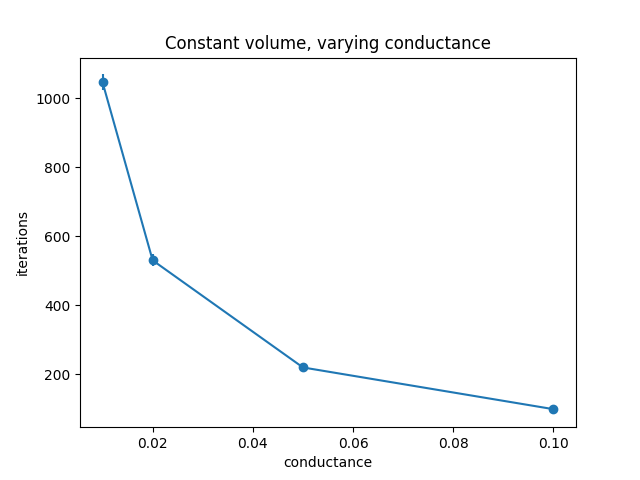
\includegraphics[width=0.8\textwidth]{const_vol.png}
            \caption{Constant volume, varying conductance: the mixing time decreases as a quadratic like curve wrt the conductance.}
            \label{fig:const_volume}
        \end{figure}
        
        \begin{figure}[h]
            \centering
            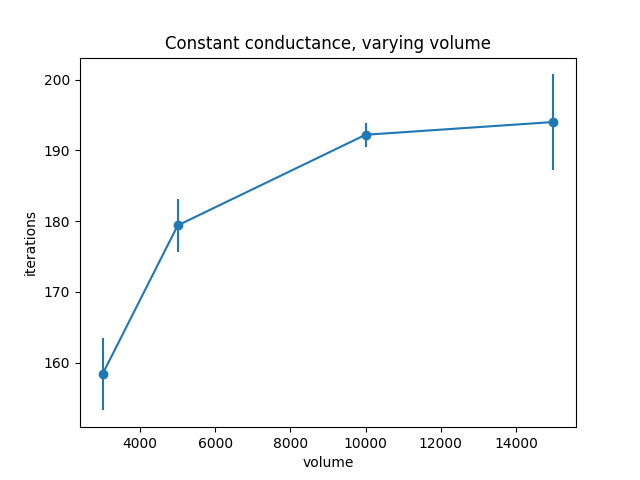
\includegraphics[width=0.8\textwidth]{const_cond.png}
            \caption{Constant conductance, varying volume: the mixing time grows with a logarithmic like curve wrt the volume.}
            \label{fig:const_conductance}
        \end{figure}
        
        As it is possible to see in Figure \ref{fig:const_conductance}, when the volume grows and the conductance remains constant, then we can observe a logarithmic growth in the mixing time (although it is not exactly a logarithm, it is interesting to see that the curve is concave and resembles a logarithm). At the same time, we can also see that in Figure \ref{fig:const_volume} it is presented the mixing time when the volume is constant and the conductance changes: it is possible to see that the increase of the conductance correspond to a decrease in the  mixing time. The curve resembles a quadratic curve $\frac{1}{x^2}$, which is our initial claim since the convergence time depends on $\frac{1}{\phi^2}$ when the volume is a constant.
        
    \subsection{R-uniform family of hypergraphs}
    
    In this experiment, we want to study the mixing time of the discrete process described in Section \ref{sec:extensions_non_d_reg_hypergraphs} applied to $r$-uniform hypergraphs. In fact, although our proof does not improve the mixing time when there is the additional assumption of $r$-uniformity, we know from \cite{continuous_laplacian_hypergraph} that actually a better upper bound exists for $r$-uniform hypergraphs: $t = O\left(\frac{\log(\text{vol}(H))}{r\phi^2}\right)$.
    
    Since the process described is discrete, it has the additional advantage of being easily simulable. Hence, we can hope to gain some insights on whether we can hope to improve the bound found for $r$ -uniform hypergraphs: in particular, we will create a family of $r$-uniform hypergraphs for different values of $r$, keeping constant both the volume and the conductance. Then, we are going to estimate the mixing time and see if the variable $r$ is inversely proportional to the mixing time. 
    
    After having generated some $r$-uniform hypergraph families with constant volume and conductance (with the same procedure as described in Section \ref{subsec:generate_hypergraph_with_desired_conductance}), we evolve the probability vector with the discrete procedure presented in Section \ref{subsubsec:preliminaries} and observe the mixing time w.r.t. the $r$-uniformity factor.
    
    \begin{figure}
        \centering
        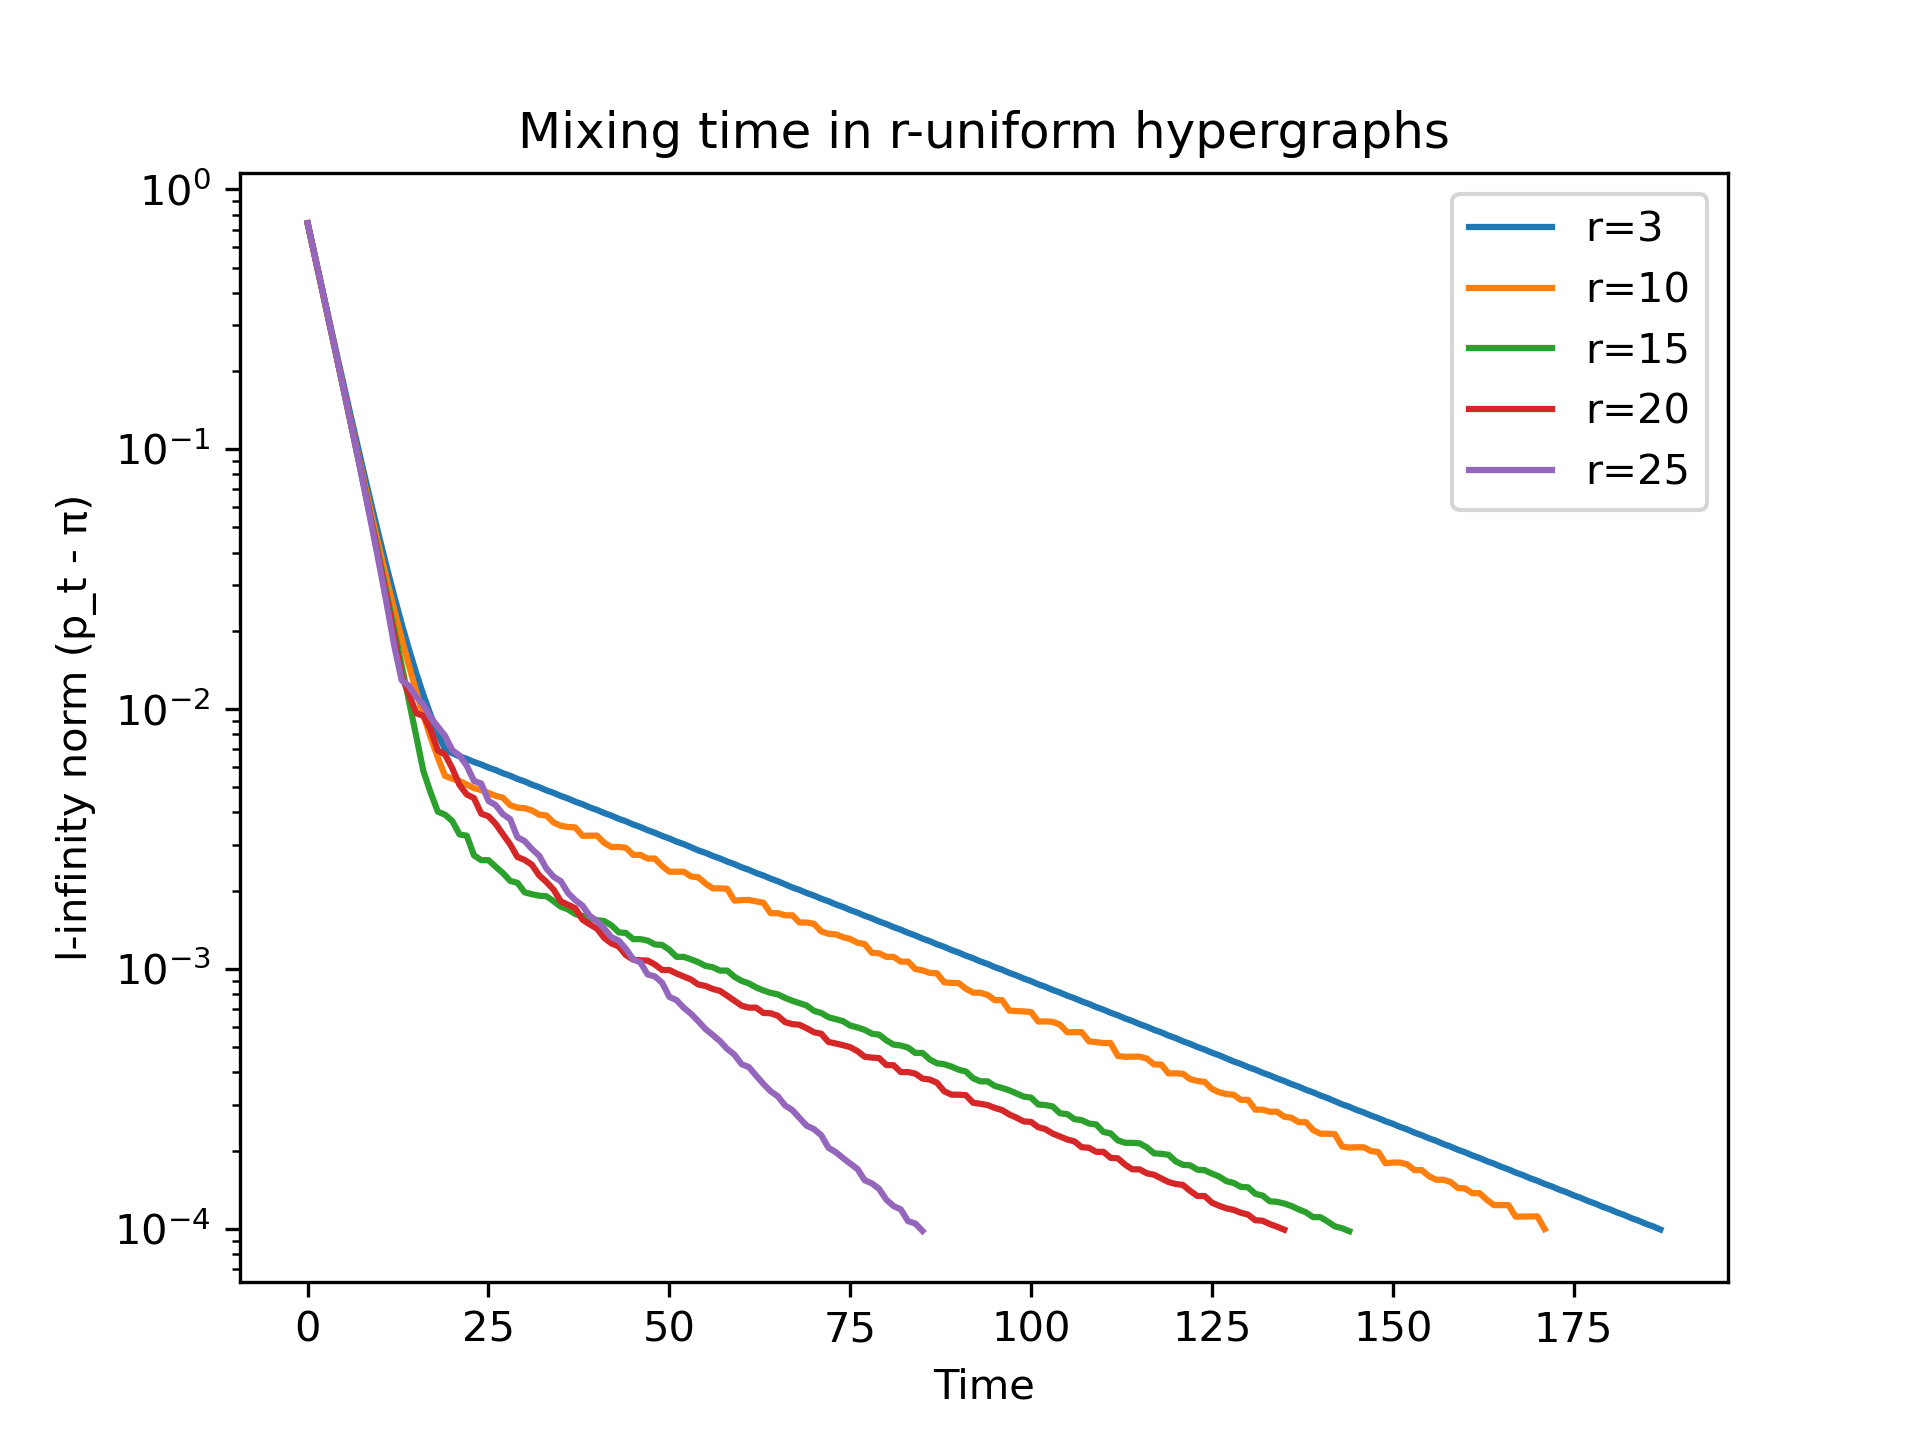
\includegraphics[width=0.8\textwidth]{img/mixing_r_uniform_hypergraph.png}
        \caption{Constant conductance, constant volume, varying $r$-uniformity factor. On the y-axis, the logarithm of the $\|\vec{p}_t-\pi\|_{\infty}$, on the $x$-axis the time $t$}.
        \label{fig:r_uniform_mixing_time}
    \end{figure}
    
    You can observe the mixing time in Figure \ref{fig:r_uniform_mixing_time}. 
    
    The plot shows the $l$-infinity norm of the vector $\| \vec{p}_t - \pi\|_{\infty}$ for different $t$ (on the $x$-axis), on a logarithmic scale. Indeed, it looks like the higher the $r$-uniformity factor, the faster the mixing time is, hence suggesting that stronger upper bounds for $r$-uniform hypergraphs can be achieved using our discrete diffusion method. This is encouraging because it might suggest that with a better analysis we might be able to prove theoretically a better mixing bound for our discrete process.
    
    
\end{document}